\documentclass[11pt]{article}
\usepackage[a4paper,margin=24mm]{geometry}
\usepackage{amsmath,amssymb,mathtools,amsthm,tikz,graphicx,longtable,booktabs,array,calc,enumitem}
\usepackage[hidelinks,hypertexnames=false]{hyperref}
\usepackage{xurl}
\usetikzlibrary{arrows.meta}
\setlength{\emergencystretch}{3em}
\providecommand{\tightlist}{}
\newcommand{\C}{\mathbb C}\newcommand{\Pp}{\mathcal P}
\newcommand{\lp}{\log^+}
\title{The actual conductor covariance:\\its evaluated outer return and original projection angles}
\author{Split-Zero research programme}
\date{21 September 2026\\SZ-20260921-009}
\begin{document}\maketitle
The complete outer covariance return is now evaluated through order
\(kq\). The original arithmetic kernel satisfies DCR26:
\[
\mathcal R\log\det H_{K,N}^{\rm ar}
=(16k-48-v)q\mathfrak C_\partial+
\log\frac{\det S_{q-1}\det S_q}{\det S_{2q-1}\det S_{2q}}
+o_{A,h}(kq).
\]
Each \(S_N\) is the specified original source-projection angle matrix,
not a freely chosen comparison. The full conductor, invariant image,
both physical integration regions, all source minima and four signs
remain. The proof pays for every omitted primary row with its full
Schur metric bound. The unprojected covariance costs only
\(O_A(q\log(q+2))=o(kq)\).
The remaining four-angle determinant must still be evaluated to obtain
the allocation coefficient; individual complex current signs also
remain uncomputed.

These are the complete new proofs CGR1--29, CGS1--22 and DCR1--27.
Earlier complete proof files are linked at their precise public editions.
The classical Gamma, orthogonal-polynomial and Jensen sources are
credited at their use. Finite exact examples check the maps and signs;
they do not substitute for the analytic arguments or identify an
off-critical zeta zero.
\tableofcontents\clearpage
\begin{figure}[ht]\centering
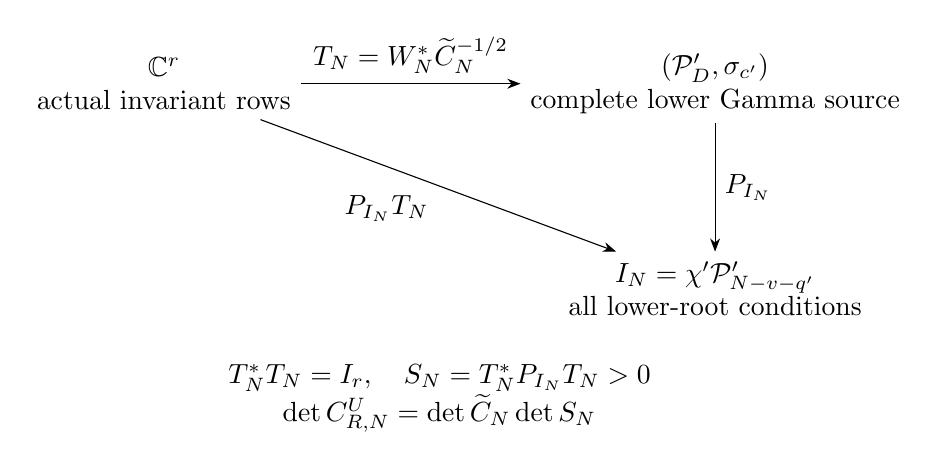
\begin{tikzpicture}[>=Stealth,every node/.style={align=center}]
\node (r) at (0,0) {$\C^r$\\actual invariant rows};
\node (d) at (7,0) {$(\Pp'_D,\sigma_{c'})$\\complete lower Gamma source};
\node (i) at (7,-2.6) {$I_N=\chi'\Pp'_{N-v-q'}$\\all lower-root conditions};
\draw[->] (r)--node[above] {$T_N=W_N^*\widetilde C_N^{-1/2}$}(d);
\draw[->] (d)--node[right] {$P_{I_N}$}(i);
\draw[->] (r)--node[below left] {$P_{I_N}T_N$}(i);
\node at (3.5,-4) {$T_N^*T_N=I_r,\quad S_N=T_N^*P_{I_N}T_N>0$\\
$\det C_{R,N}^U=\det\widetilde C_N\det S_N$};
\end{tikzpicture}
\caption{Exact maps CGS13--20. The first arrow is the displayed isometry
from the actual invariant covariance, with its full conductor inverse.
The second is the unchanged source projection. CGS17 bounds the
unprojected determinant by \(O_A(q\log(q+2))\); DCR26 preserves the
remaining angle determinants at all four cutoffs. No geometric angle is
drawn or assigned a value. The complete primary-decomposition diagram
appears with DCR5--8.}
\end{figure}

\clearpage\part{The original covariance and its conductor-pole filtration}
\section{The original invariant covariance and its conductor-pole filtration}\label{the-original-invariant-covariance-and-its-conductor-pole-filtration}

21 September 2026. Independent continuation of CG29--32. All coefficient rows below are the actual invariant rows surviving the complete low-jet constraint. No replacement of their metric, their source projection or their original period is made.

This calculation proves two quantitative statements. First, the sum of the positive logarithmic eigenvalues of the original invariant covariance, relative to its specified original coefficient form, is \(O_A(q\log(q+2))=o(kq)\). Second, the remaining graph-covariance changes in CG32 can be restricted to the \textbf{actual invariant rows that vanish at the specified conductor poles}, with error \(O_A(q\sqrt{k}\log^2(q+2))=o(kq)\). The removed rows are controlled by proved metric bounds before their number is used. On the retained rows the entire conductor covariance has a quadratic-form upper bound \(\exp(o(q))\) in that coefficient form. Its small eigenvalues and its comparison with the outer-ideal covariance remain to be evaluated.

\subsection{1. Every row and every analytic function comes from the original data}\label{every-row-and-every-analytic-function-comes-from-the-original-data}

Retain KF1--55, CG1--32, the complete OCF invariant construction, and \[
N\in\{q-1,q,2q-1,2q\},\quad L=N-q,
D=N-v,\quad r=8k-32-v+s_k.
\tag{CGR1}
\] Let \(Z\in\mathbb C^{r\times q}\) contain the actual coefficient rows obtained in CG29--30. It is supported on the OCF strip \(E_k^{\rm strip}\), has full row rank, and each row annihilates the entire degree-\(<v\) polynomial space. It is a linear combination of the complete columns \(J_R=S_kZ_k\), followed by the exact elimination of \(\operatorname{im}B_{\mathcal L}\). Its reference coefficient form is \[
R_Z=ZZ^*>0.
\tag{CGR2}
\] This is only a fixed reference used to compare matrices. Every actual Gamma metric below remains unchanged.

For a row \(z=(z_\alpha)\) in this original row space define \[
F_z(w)=\sum_{\alpha=1}^qz_\alpha e^{\beta_\alpha w},\qquad
G_z(w)=F_z(w)/E_A(w).
\tag{CGR3}
\] Since the row kills all degree-\(<v\) polynomials, \(F_z^{(j)}(0)=0\) for \(j<v\). Thus \(G_z\) is holomorphic at zero. The numerator is the original invariant biform restricted to the original exponential curve. OCF17 supplies an invariant lift also for the strip representative: subtracting its conductor part stays inside the invariant image. No arbitrary exponential numerator has been inserted.

For every polynomial \(p\), finite differentiation gives the exact duality \[
[p(\partial_w)F_z(w)]_{w=0}
=[(\mathcal T_Ap)(\partial_w)G_z(w)]_{w=0}.
\tag{CGR4}
\] For a single monomial this is Leibniz's formula for \(F_z=E_AG_z\); linearity proves the general case. Consequently the complete target observation is \[
\ell_z(\eta)=
[\eta(\partial_w)\chi'(\partial_w)G_z(w)]_{w=0}.
\tag{CGR5}
\] Indeed KF8--10 give \(\mathcal T_A\mathcal R(\chi'\eta)=\chi'\eta\), and CGR4 gives precisely CG29's coefficient row on every low polynomial \(\eta\). The extension CGR5 annihilates the \textbf{entire} relation: \[
\ell_z(\mathcal U_Ah)
=[(\mathcal T_A(\chi h))(\partial_w)G_z]_{0}
=[(\chi h)(\partial_w)F_z]_{0}=0,
\tag{CGR6}
\] because every exponent \(\beta_\alpha\) is a root of the full original \(\chi\). Thus it is the actual quotient observation at every cutoff, not an extension chosen for a norm estimate.

\subsection{2. The exact original Gamma covariance, with its projection retained}\label{the-exact-original-gamma-covariance-with-its-projection-retained}

Let \(A=A_{D,1}\) be the complete WCF6 matrix from the upper-center Gamma frame \(\phi_{v,c},\ldots,\phi_{N,c}\) to the lower-center frame \(\phi_{0,c'},\ldots,\phi_{D,c'}\). Its entries and every phase are unchanged. Let \(B_F\in\mathbb C^{r\times(D+1)}\) have entries \[
(B_F)_{j,n}=[\phi_{v+n,c}(\partial_w)F_{z_j}(w)]_{0}.
\tag{CGR7}
\] In the lower-center orthonormal coefficient space let \(P_I\) be the orthogonal projection onto the exact polynomial subspace \[
I_N=\chi'\mathcal P'_{L+g}\subset\mathcal P'_D.
\tag{CGR8}
\] The target observation covariance is exactly \[
\boxed{C_{R,N}^U=B_FA^{-1}P_I(A^{-1})^*B_F^*.}
\tag{CGR9}
\] To prove it, CGR4 on the source Gamma basis gives the lower functional row \(B_FA^{-1}\). Its restriction to \(I_N\) is its composition with the orthogonal projection \(P_I\); the squared Gram of those restricted rows is CGR9. Multiplication by \(\chi'\) is exactly the isometry from the weighted target source into \(I_N\). CGR6 shows that taking the complete quotient afterward leaves that observation covariance unchanged. The projection \(P_I\), of codimension \(q'\), is present throughout.

Set \(R_y=k\sqrt{\delta^2+\gamma^2}\) and retain the exact finite root-evaluation bound from KF33, \[
V_N=\frac{qe^2}{M_\sigma}(N+1)^{3/2}(2N+1)^{R_y+1}.
\tag{CGR10}
\] Then \(B_FB_F^*\preceq V_NR_Z\). This follows by writing the rows as the original coefficient rows times the complete root-evaluation matrix; discarding the first \(v\) source columns does not increase its norm. The bound itself follows from the generating function on radius \(N/(N+1)\), as proved in KF33 and CG23.

With \(M_D,J_D\) exactly as in CG23, the WCF19d exterior estimate gives, for each \(1\le j\le r\), \[
\prod_{i=1}^j\lambda_i
\le V_N^j M_D^{2(D+1-j)}e^{2J_D},
\tag{CGR11}
\] where \(\lambda_1\ge\cdots\ge\lambda_r>0\) are the eigenvalues of \(R_Z^{-1/2}C_{R,N}^UR_Z^{-1/2}\). In fact factor its rectangular Gram matrix as \(R_Z^{-1/2}B_FA^{-1}P_I\), apply the exterior norm to each factor, and use that an orthogonal projection contracts every exterior norm. The product of the largest \(j\) squared singular values is the displayed left side. Taking the largest partial logarithmic sum proves \[
\boxed{\sum_{i=1}^r\log^+\lambda_i
\le r\log^+V_N+2(D+1)\log M_D+2J_D
=O_A(q\log(q+2))=o(kq).}
\tag{CGR12}
\] Here \(r=O(k)\), \(\log V_N=O_A(k\log(q+2))\), and the WCF quantities have their already proved orders. This controls every positively amplified covariance direction jointly. It neither bounds the negative logarithms by the same expression nor assumes the retained projection is an identity.

\subsection{3. Finite global bounds needed before eliminating pole directions}\label{finite-global-bounds-needed-before-eliminating-pole-directions}

These bounds will pay for the actual eliminated directions, including their angles. Let \(a_*^{\rm piv}\ne0\) be the original leading conductor coefficient selected in OCF5, and put \[
C_A=1+A_1/|a_*^{\rm piv}|,\qquad
B_{\rm val}=qM_\sigma
\left(\frac{2q+R_y}{2\delta}\right)^{2(q-1)}.
\tag{CGR13}
\] Each OCF6 coefficient elimination has coefficient \(\ell^1\) operator norm at most \(C_A\): it subtracts a scalar coefficient times the full shifted conductor polynomial divided by its actual pivot. There are \(q'\) steps. Hence its exact strip reduction satisfies \(\|N_k\|_2\le\sqrt q C_A^{q'}\). For any original strip row \(z\), and any conductor coefficient vector \(M_Au\), \[
\|z-M_Au\|_2\ge\|z\|_2/\|N_k\|_2.
\tag{CGR14}
\] This follows from \(N_kM_A=0\) and \(N_kz=z\) in the identical strip positions. It is a quantitative consequence of the actual full conductor elimination, not an assumption about the angle of the invariant image.

The complete source covariance in root-value coordinates is at least \(B_{\rm val}^{-1}I_q\), by the explicit Lagrange interpolation estimate KF34. The lower bound can also be read directly from the inverse norm of the interpolation polynomials: each root separation has modulus at least \(2\delta\), and successive multiplication by \(y-\omega\) has Gamma norm at most \(2q+R_y\) on the relevant degrees. The sum of their squared norms is exactly bounded by CGR13.

The orthogonal complement of \(I_N\) is the span of evaluations at every original lower root. Apply CGR4 to these evaluation rows. WCF21--22 gives their images under \(A\) as exactly the complete upper conductor rows. All their first \(v\) Gamma coefficients, like those of \(F_z\), vanish. Consequently the distance defining the left side of CGR9 is at least the distance of the original source row to the conductor image divided by \(\|A\|\). Using CGR14 and the full source lower bound proves \[
l_{U,N}R_Z\preceq C_{R,N}^U\preceq u_{U,N}R_Z,
\quad
l_{U,N}=\frac1{M_D^2 B_{\rm val}q C_A^{2q'}},\qquad
u_{U,N}=V_N M_D^{2D}e^{2J_D}.
\tag{CGR15}
\] For the upper bound use CGR11 at \(j=1\). In particular \(\log^+u_{U,N}+\log^+(1/l_{U,N})=O_A(q\log(q+2))\). No lower eigenvalue is asserted to be of order one.

For clarity, the corresponding outer-ideal covariance has finite bounds in the \textbf{same} reference form, not a newly chosen observation frame. At \(N_0=q-1\), CG24 proves \(C_{R,N_0}^d=C_{R,N_0}^U\). The outer observation is fixed polynomial remainder followed by \(A_R\), so enlarging its source adds nonnegative rank-one covariance terms. Thus \(C_{R,N}^d\succeq l_{U,N_0}R_Z\) at all later cutoffs.

Here are explicit upper constants. Write \(M=L+g\) for the target source degree, \(c'=k/2-4\), and keep CG6's finite domain. Put \[
\begin{split}
R_d&=\max\{1,|c'|+q/r_*\},\qquad t_d=2R_d,\\
B_{\rm rem}(M)&=g2^g(1+R_d)^g\sqrt{M+1}\,t_d^M,\\
h_-(M)&=\frac{C_Le^{-\pi(q+1)}(q^2-R_y^2)^{q'}}
{(M+1)^2(2M+1)64^M(1+|c'|+q)^{2M}},\\
h_+^0&=gM_\sigma(4q+2+R_y+|c'|)^{2q}.
\end{split}\tag{CGR16}
\] Ordinary remainder by \(d_A/a_A\) on the coefficient vectors of \(1,S',\ldots,S'^M\) has norm at most \(B_{\rm rem}(M)\). To prove it, use the exact Cauchy remainder formula on \(|S'|=t_d\). Its denominator has modulus at least \((t_d/2)^g\); its monic coefficient sum is at most \((1+R_d)^g\). The coefficient sum of its divided difference is at most \(g t_d^{g-1}(1+R_d)^g\). Contour length supplies \(t_d\), and a source polynomial has boundary maximum at most \(\sqrt{M+1}t_d^M\) times its coefficient norm. This proves the bound, including repeated roots, since the contour remainder retains all jets.

The complete source Gram \(H_M\) in this coefficient frame obeys \(H_M\succeq h_-(M)I\). On \(q\le y\le q+1\), paired lower roots give \(|\chi'(c'+iy)|^2\ge(q^2-R_y^2)^{q'}\), and CG4's Gamma density bound contributes \(C_Le^{-\pi(q+1)}\). Expanding on \([0,1]\) in shifted Legendre polynomials, as in CG17, bounds the coefficient norm after the substitution \(S'=c'+i(q+x)\) by \((M+1)\sqrt{2M+1}\,8^M(1+|c'|+q)^M\) times the interval \(L^2\) norm. Squaring gives \(h_-(M)\). The low Gram \(H_{g-1}\) has norm at most \(h_+^0\): multiply its monomial columns by all \(q'\) original root factors and use CG11's upper bound on each, then sum their squared norms. All these products have degree at most \(q\).

At the first cutoff \(C_{R,N_0}^U=A_RH_{g-1}^{-1}A_R^*\), hence \(A_RA_R^*\preceq h_+^0u_{U,N_0}R_Z\). Applying the complete remainder bound to the high source covariance now proves \[
l_dR_Z\preceq C_{R,N}^d\preceq u_{d,N}R_Z,
\quad l_d=l_{U,N_0},\qquad
u_{d,N}=\frac{B_{\rm rem}(M)^2h_+^0u_{U,N_0}}{h_-(M)}.
\tag{CGR17}
\] Every logarithmic bound in CGR17 has size \(O_A(q\log(q+2))\), since \(M\le q+g=O(q)\), \(g=O(k)\), and \(R_d=O_A(q)\). These deliberately coarse global constants are used only on the few rows removed next.

\subsection{4. An exact growing family of conductor-pole constraints}\label{an-exact-growing-family-of-conductor-pole-constraints}

Retain the full WCF function and the original center difference: \[
w(t)=-i\arctan t,\quad
g_A(t)=t^{-v}e^{-4w(t)}E_A(w(t)),\quad
g_A(0)=g_0=(-i)^v\mu_v/v!\ne0.
\tag{CGR18}
\] The powers and logarithm are their analytic branches at \(t=0\), on the unit disk. For the original row \(z\), its upper generating function and the lower generating function of \(G_z\) satisfy \[
\begin{split}
f_z(t)&=t^{-v}(1+t^2)^{-1/4}e^{-cw(t)}F_z(w(t)),\\
H_z(t)&=(1+t^2)^{-1/4}e^{-c'w(t)}G_z(w(t)),\qquad
f_z(t)=g_A(t)H_z(t).
\end{split}\tag{CGR19}
\] The exact coefficients of \(H_z\) are \([p_n((\partial_w-c')/i)G_z(w)]_0/n!\). This follows by applying the original Gamma generating function to the linear functional. The factors \(c,c'\), \(i\), and \(e^{-4w}\) all remain. The apparent singularity of \(f_z\) at zero is removable because the first \(v\) source coefficients vanish.

Put \[
\eta=k^{-1/2},\quad \rho=1-2\eta,\quad
R_1=1-\eta,\quad R_2=1-\eta/2,
\tag{CGR20}
\] which belong to \((0,1)\) for the original \(k\ge9\). Define \[
M_g=\max\left\{1,|g_0|,
2^vA_1e^{2\pi\gamma}
\left(\frac{1+R_2}{1-R_2}\right)^{4\delta}\right\},
\quad J_g=\log(M_g/|g_0|)\ge0.
\tag{CGR21}
\] WCF7--8 bounds \(|g_A|\) by \(M_g\) on \(|t|\le R_2\). Let its zeros in \(|t|<R_1\) be \(\zeta\), with their actual multiplicities \(m_\zeta\), and let \(H_k=\sum m_\zeta\). Jensen's finite disk formula gives \[
H_k\le\frac{J_g}{\log(R_2/R_1)}\le\frac{2J_g}{\eta}
=O_A(\sqrt{k}\log(k+2)).
\tag{CGR22}
\] Indeed every such zero contributes at least \(\log(R_2/R_1)\) to the Jensen sum at \(R_2\), while the boundary mean is at most \(\log M_g\). The formula follows by factoring its zeros and applying the mean-value formula to the logarithm of the remaining nonzero analytic factor; this is the same full proof used in OR9. The second inequality follows from \(\log(R_2/R_1)\ge(R_2-R_1)/R_2\ge\eta/2\).

Define a subspace \textbf{inside the original invariant row space} by \[
\mathcal W_k^0=
\{z:\ F_z^{(j)}(w(\zeta))=0
\text{ for every }\zeta\text{ above and }0\le j<m_\zeta\}.
\tag{CGR23}
\] Its exact codimension \(h_k\) is the rank of the displayed finite matrix of actual values \(\beta_\alpha^j e^{\beta_\alpha w(\zeta)}\) after multiplication by \(Z\); in particular \(h_k\le H_k\). Every derivative and point is specified by the original conductor and invariant rows. Since \(w'(t)=-i/(1+t^2)\ne0\), these constraints say exactly that the numerator \(f_z\) cancels the indicated zeros of \(g_A\) with their full multiplicities. There is no unspecified generic rank.

\subsection{5. The complete projected covariance on those rows has sub-q upper cost}\label{the-complete-projected-covariance-on-those-rows-has-sub-q-upper-cost}

Let \(B(t)\) be the finite disk Blaschke product of the zeros in CGR22, with factors \(R_1(t-\zeta)/(R_1^2-\bar\zeta t)\), repeated with their multiplicities. Its boundary modulus on \(|t|=R_1\) is one and \(|B(0)|\le1\). Both \(f_z/B\) and \(g_A/B\) are holomorphic there for \(z\in\mathcal W_k^0\), and the second has no interior zero. The maximum principle gives \(\max|f_z/B|\le\max_{|t|=R_1}|f_z(t)|\). Also \(u(t)=\log(M_g/|g_A(t)/B(t)|)\) is nonnegative harmonic in that disk, with \(u(0)\le J_g\). Its Poisson integral gives \[
u(t)\le\frac{R_1+\rho}{R_1-\rho}u(0)
\le\frac{2J_g}{\eta}\qquad(|t|\le\rho).
\tag{CGR24}
\] For the inequality, the Poisson kernel on any intermediate circle of radius \(R< R_1\) is at most \((R+|t|)/(R-|t|)\); its average of \(u\) is \(u(0)\). Let \(R\) tend to \(R_1\). Boundary zeros of \(g_A\), if any, do not affect this interior argument or the maximum principle.

The numerator bound retaining its original coefficient norm is \[
\max_{|t|=R_1}|f_z(t)|
\le F_k\|z\|_2,\qquad
F_k=R_1^{-v}(1-R_1^2)^{-1/4}\sqrt q
\exp\{R_y\operatorname{arctanh}R_1\}.
\tag{CGR25}
\] In fact the original center factor cancels \(e^{cw}\) in each original exponential; the remaining exponent has modulus at most \(R_y|w|\), and \(|w(t)|\le\operatorname{arctanh}R_1\). Cauchy--Schwarz on all \(q\) unchanged coefficients proves CGR25. Using \(M_g\ge1\), CGR24--25 therefore bound the full lower generating function by \(\max_{|t|\le\rho}|H_z(t)|\le F_ke^{2J_g/\eta}\|z\|_2\). Its coefficient of degree \(n\) has modulus at most this quantity times \(\rho^{-n}\). The normalized Gamma functional coefficient multiplies that coefficient by \(\rho_n/\sqrt{M_\sigma}\), where \(\rho_n^2=n!/(1/2)_n\le2n+1\). Summing every source coefficient through \(D\), and then retaining the original orthogonal projection, proves \[
\boxed{C_{R,N}^U\big|_{\mathcal W_k^0}
\preceq e^{\varepsilon_{k,N}}R_Z\big|_{\mathcal W_k^0},}
\quad
\varepsilon_{k,N}=
\log\frac{(D+1)(2D+1)}{M_\sigma}+2\log F_k
+\frac{4J_g}{\eta}+2D\log(1/\rho).
\tag{CGR26}
\] An upper bound using \(\max(0,\varepsilon_{k,N})\) is available if a nonnegative allowance is desired. Explicitly \[
\varepsilon_{k,N}
=O_A(k^{3/2}+k\log(k+2)+\sqrt{k}\log(k+2))=o(q).
\tag{CGR27}
\] Here \(D\le2q\), \(\log(1/\rho)=O(k^{-1/2})\), \(\operatorname{arctanh}R_1=O(\log k)\), and \(J_g=O_A(\log k)\). The proof never replaces the projected norm by an equality with the full norm; the full norm is used only for its valid upper bound.

\subsection{6. The actual allocation loses only o(kq) when these poles are removed}\label{the-actual-allocation-loses-only-okq-when-these-poles-are-removed}

Choose a basis orthonormal for the fixed coefficient form \(R_Z\), whose first \(r-h_k\) rows span the exact subspace CGR23. Use that same basis at both high cutoffs and for both \(U,d\). In its block decomposition the determinant equals the determinant of the first restriction times the determinant of its attained Schur complement. Denote the covariance change on the first restriction by \(\Delta_{R,N}^0\).

Congruence and attained minimization transport CGR15 and CGR17 to those Schur complements: every eigenvalue for \(U\) lies in \([l_{U,N},u_{U,N}]\), and every one for \(d\) lies in \([l_d,u_{d,N}]\). Their rank is exactly \(h_k\). Therefore \[
\boxed{|\Delta_{R,N}-\Delta_{R,N}^0|
\le h_k\max\left\{
\log^+\frac{u_{U,N}}{l_d},
\log^+\frac{u_{d,N}}{l_{U,N}}\right\}
=O_A(q\sqrt{k}\log^2(q+2))=o(kq).}
\tag{CGR28}
\] This is where the number of pole directions is used. Their complete metric costs were bounded first, so no unproved angle estimate or deletion by rank is concealed in CGR28. The coefficient basis is only an exact fixed change of frame and its determinant cancels in each covariance ratio.

Combining with the already evaluated full-volume error CG32 gives \[
\boxed{\mathcal G_K
=-\Delta_{R,2q-1}^0-\Delta_{R,2q}^0+o_A(kq).}
\tag{CGR29}
\] For a finite bound, add CG32's displayed finite right side to the two finite right sides of CGR28. Thus the remaining leading allocation is now localized to an explicitly defined, original invariant row space with every selected conductor pole canceled. It still has dimension \(r-O_A(\sqrt{k}\log(k+2))\). CGR26--27 control its upper covariance quadratic form. The lower spectrum and the signed comparison with \(C_{R,N}^d\) on this space are not evaluated here; an upper bound alone cannot assign their determinant ratio or an RH conclusion.

\subsection{Sources and exact reading coverage}\label{sources-and-exact-reading-coverage}

OCF1--26, \emph{An exact conductor frame and a fixed invariant-generator recursion}, was read completely for this continuation. CGR3 and CGR14 use its exact strip representatives, conductor columns and invariant certificates. The \href{https://github.com/KokunoYumeto/zeta-function-research-reader/blob/5992ad50c0f2a06921f1fcaded7b4e38097c0739/workbenches/splitzero-tandem/continuations/20260920-original-kernel-mixed-determinants/providers/ORIGINAL_CONDUCTOR_STRIP_FRAME.tex\#L27}{complete pinned proof file} is byte-verified in the root public-source receipt.

KF1--55 and CG1--32 were read completely. This continuation retains their actual \(A_R\), full low constraint, frame and source. Their complete source must accompany publication before a live link is claimed.

WCF4--13, WCF19a--f and WCF20--22 are used from the \href{https://github.com/KokunoYumeto/zeta-function-research-reader/blob/52274804051e325c8a6ef69c17b3958cc2caba0a/workbenches/splitzero-tandem/continuations/20260920-gamma-and-finite-derivative/providers/WEIGHTED_CONDUCTOR_FORWARD.tex}{pinned complete proof file}, whose byte identity was checked in the CG source. The cited portions were read directly. The Gamma generating function is NIST DLMF \href{https://dlmf.nist.gov/18.23.E7}{18.23.7}, with recurrence \href{https://dlmf.nist.gov/18.22.E8}{18.22.8}, by T. H. Koornwinder, R. Wong, R. Koekoek, R. F. Swarttouw and W. P. Reinhardt, version 1.2.8. Its original TeX encodings are retained in \nolinkurl{graph_primary_sources/}. The generating function is applied explicitly in CGR19 with both original centers and their exact phase. Jensen's zero count is the classical formula of J. L. W. V. Jensen, \emph{Sur un nouvel et important théorème de la théorie des fonctions} (1899), \href{https://doi.org/10.1007/BF02417878}{DOI 10.1007/BF02417878}; the finite proof used here is included in OR9 and recalled in CGR22. The disk-product and harmonic inequalities needed in CGR24 are proved above rather than supplied as missing analytic assumptions.

The independent checker \nolinkurl{check_invariant_covariance.py} passed 96 exact tests of CGR3--9, with v=0 and v=1 finite-shift fixtures, both retained Gamma centers, the physical complex phase, the complete relation minimum and the original source projection. Deleting that projection or changing the phase fails the respective negative control. These finite checks do not replace the analytic proofs of CGR10--29.

The exact earlier proof files are \href{https://github.com/KokunoYumeto/zeta-function-research-reader/blob/0fd693c844aad9117e30ec447c59864a28af10f3/workbenches/splitzero-tandem/continuations/20260921-native-spectral-real-pair/003/ACTUAL_KERNEL_FILTRATION_AND_GRAPH.tex\#L12}{KF1--55}, \href{https://github.com/KokunoYumeto/zeta-function-research-reader/blob/0fd693c844aad9117e30ec447c59864a28af10f3/workbenches/splitzero-tandem/continuations/20260921-native-spectral-real-pair/003/COMPLETE_CONDUCTOR_GRAPH_METRIC.tex}{CG1--32}, and \href{https://github.com/KokunoYumeto/zeta-function-research-reader/blob/0fd693c844aad9117e30ec447c59864a28af10f3/workbenches/splitzero-tandem/continuations/20260921-native-spectral-real-pair/003/COMPLETE_CONDUCTOR_ROOT_GEOMETRY.tex\#L38}{OR1--25}. CGR and CGS are reproduced completely in this edition.


\clearpage\part{The original strip and its projection-angle loss}
\section{The original strip has linear elimination depth; its leading native covariance loss is an original projection angle}\label{the-original-strip-has-linear-elimination-depth-its-leading-native-covariance-loss-is-an-original-projection-angle}

21 September 2026. Independent continuation of CGR1--29. The full original conductor, invariant image, Gamma source and quotient minimum are retained. The results below concern the actual row space of CG29--30 at all four original cutoffs. They quantify the source contribution and locate the remaining leading covariance in an exact projection. They do not assign the remaining projection determinant a value.

\subsection{1. The exact conductor elimination has depth at most 10k}\label{the-exact-conductor-elimination-has-depth-at-most-10k}

Use the entire OCF4 conductor \[
A=\sum_{r,s=0}^{8}a_{rs}e_{rs}^{(8)},\qquad
(r_0,s_0)=\max_{\mathrm{lex}}\{(r,s):a_{rs}\ne0\},\qquad
a_*=a_{r_0s_0},\qquad A_1=\sum_{r,s}|a_{rs}|.
\tag{CGS1}
\] The subscripts \(r_0,s_0\) here denote the actual leading monomial, not the earlier residual-rank symbol. Set \[
B_A^{\mathrm{step}}=\frac{A_1-|a_*|}{|a_*|},\qquad
C_A^{\mathrm{path}}=1+B_A^{\mathrm{step}}=\frac{A_1}{|a_*|}\ge1.
\tag{CGS2}
\] Give the original coefficient position \((a,b)\in\{0,\ldots,k\}^2\) the integer height \(h(a,b)=9a+b\). OCF6 replaces a pivot coefficient at \((r_0+i,s_0+j)\) by the entire sum \[
-\sum_{(r,s)\ne(r_0,s_0)}\frac{a_{rs}}{a_*}
   e_{r+i,s+j}^{(k)}.
\tag{CGS3}
\] Every nonzero term has strictly smaller height. If \(r=r_0\), its decrease is \(s_0-s\ge1\). If \(r<r_0\), the decrease is \(9(r_0-r)+(s_0-s)\ge9-8=1\). Every destination remains in the original coefficient box, since \(0\le i,j\le k-8\) and \(0\le r,s\le8\). Thus a path of successively replaced coefficients has length at most \(10k\); coefficients are never removed from the original box to obtain this bound.

For completeness, expand the reduction of one basis column as the sum over all its substitution paths, stopping each path when it reaches the actual strip. At a substituted node the sum of absolute edge weights is \(B_A^{\mathrm{step}}\). The sum of absolute weights of all terminal paths of a specified length \(j\) is consequently at most \((B_A^{\mathrm{step}})^j\), by induction on the successive levels. The triangle inequality therefore bounds the total output column norm by \(\sum_{j=0}^{10k}(B_A^{\mathrm{step}})^j\), which is at most \((1+B_A^{\mathrm{step}})^{10k}\). The latter assertion follows by expanding the binomial and using \(\binom{10k}{j}\ge1\). When \(B_A^{\mathrm{step}}=0\), the same expression is one. The exact strip map therefore obeys \[
\boxed{\|N_k\|_{1\to1}\le(C_A^{\mathrm{path}})^{10k},\qquad
\|N_k\|_{2\to2}\le\sqrt q(C_A^{\mathrm{path}})^{10k}.}
\tag{CGS4}
\] This computes a quantitative bound for the existing OCF elimination; the order and coefficients of that elimination have not been changed. The second inequality uses \(\|u\|_2\le\|u\|_1\) on the output and \(\|f\|_1\le\sqrt q\|f\|_2\) on its original input.

In the identical strip positions, \(N_kz=z\) and \(N_kM_A=0\). Thus the complete conductor image has the following proved angle from every original strip coefficient vector: \[
\boxed{\operatorname{dist}_{\ell^2}(z,\operatorname{im}M_A)
\ge\frac{\|z\|_2}{\sqrt q(C_A^{\mathrm{path}})^{10k}}.}
\tag{CGS5}
\] Apply \(N_k\) to \(z-M_Au\), use CGS4, and take the infimum over all original conductor coefficients \(u\) to prove the formula. Consequently CGR15 remains valid with the path-based lower constant \[
l_{U,N}^{\mathrm{path}}=
\left[M_D^2B_{\mathrm{val}}q
          (C_A^{\mathrm{path}})^{20k}\right]^{-1}.
\tag{CGS6}
\] The \(B_{\mathrm{val}}\) in this statement is still the complete \(q\)-root interpolation constant of CGR13. The original source projection is still present; CGS5 does not erase that factor. One may take the larger of CGS6 and the prior lower constant at each finite cutoff. The new path bound improves the growth exponent as \(k\) increases; it need not be the smaller numerical bound for the first few allowed values of \(k\).

\subsection{2. The sparse strip has a smaller interpolation constant before projection}\label{the-sparse-strip-has-a-smaller-interpolation-constant-before-projection}

There are exactly \[
n_E=|E_k^{\mathrm{strip}}|=q-q'=16k-48
\tag{CGS7}
\] original roots in the strip. Their physical coordinates are \[
y_{ab}=(\beta_{ab}-c)/i=(2b-k)\gamma-i(2a-k)\delta,
\quad (a,b)\in E_k^{\mathrm{strip}},\quad c=k/2.
\tag{CGS8}
\] Every one has modulus at most \(R_y=k\sqrt{\delta^2+\gamma^2}\). Every pair has separation at least \(2\delta\), because \(0<\delta<1/2\), \(\gamma>2\), and distinct pairs differ in at least one coordinate. In the original Gamma norm define its Lagrange polynomials by \[
L_\alpha(y)=\prod_{\beta\in E_k^{\mathrm{strip}},\ \beta\ne\alpha}
\frac{y-y_\beta}{y_\alpha-y_\beta}.
\tag{CGS9}
\] These interpolate precisely the strip roots. No lower-lattice root is inserted in this interpolation and none is dropped from the later source projection.

Successive application of CG11 to every displayed factor gives \[
\|L_\alpha\|_\sigma^2
\le M_\sigma\left(\frac{2n_E+R_y}{2\delta}\right)^{2(n_E-1)},
\qquad
B_E=n_EM_\sigma
\left(\frac{2n_E+R_y}{2\delta}\right)^{2(n_E-1)}.
\tag{CGS10}
\] Indeed the degree before any multiplication is at most \(n_E-2\), so CG11 bounds that multiplication norm by \(2n_E+R_y\); each denominator has modulus at least \(2\delta\), and the norm of the constant polynomial is exactly \(\sqrt{M_\sigma}\).

Let \(E_{E,N}\) evaluate the complete upper Gamma frame of degrees \(0,\ldots,N\) at these actual roots. Since \(n_E-1\le q-1\le N\), the polynomials CGS9 form a right inverse of this evaluation map at every original cutoff. Its squared operator norm is at most the sum of the squared column norms, namely \(B_E\). For a row \(z\), applying that right inverse to \(zE_{E,N}\) gives \[
\|zE_{E,N}\|_2^2\ge B_E^{-1}\|z\|_2^2.
\tag{CGS11}
\] This proves the lower bound without a Vandermonde determinant estimate.

The actual rows in \(Z\) are supported on this strip and annihilate all polynomials of degree below \(v\). Their first \(v\) Gamma functional coefficients consequently vanish exactly. Thus removing those zero columns leaves the identical row norm, and CGR7 satisfies \[
\boxed{B_E^{-1}R_Z\preceq B_FB_F^*\preceq V_NR_Z.}
\tag{CGS12}
\] The right inequality is CGR10. The left inequality uses exactly the unchanged sparse rows of the invariant image. It is not a statement about the covariance after projecting away the lower root evaluations.

\subsection{3. The complete unprojected native covariance has only o(kq) determinant cost}\label{the-complete-unprojected-native-covariance-has-only-okq-determinant-cost}

Retain \(A=A_{D,1}\), \(D=N-v\), and define \[
W_N=B_FA^{-1},\qquad
\widetilde C_{R,N}=W_NW_N^*,\qquad
C_{R,N}^U=W_NP_IW_N^*.
\tag{CGS13}
\] Every matrix is in the original lower-center Gamma frame; CGR9 proves the last equality with the original orthogonal projection \(P_I\) onto \(\chi'\mathcal P'_{L+g}\). The forward WCF bound \(\|A\|\le M_D\) and CGS12 prove \[
\widetilde C_{R,N}\succeq
           (M_D^2B_E)^{-1}R_Z.
\tag{CGS14}
\] For each \(j\le r\), the same exterior argument as CGR11, now without a projection, gives \[
\prod_{i=1}^j\widetilde\lambda_i
\le V_N^jM_D^{2(D+1-j)}e^{2J_D},
\tag{CGS15}
\] where the ordered eigenvalues are those relative to \(R_Z\). All factors come from the original operator and the exact strip rows.

Set \[
\begin{split}
K_{-,N}&=r\log^+(M_D^2B_E),\\
K_{+,N}&=r\log^+V_N+2(D+1)\log M_D+2J_D,\\
K_N&=\max\{K_{-,N},K_{+,N}\}.
\end{split}\tag{CGS16}
\] Taking the determinant in CGS14 bounds its logarithm below by \(-K_{-,N}\). Taking the largest partial sum of the ordered logarithms in CGS15 bounds its positive logarithmic part by \(K_{+,N}\), hence its whole logarithm above by that number. We have therefore evaluated the size of the complete source contribution: \[
\boxed{\left|\log\frac{\det\widetilde C_{R,N}}{\det R_Z}\right|
\le K_N=O_A(q\log(q+2))=o(kq).}
\tag{CGS17}
\] To check the stated order, \(r=O(k)\), \(n_E=O(k)\), \(R_y=O_A(k)\), \(\log B_E=O_A(k\log(k+2))\), \(\log V_N=O_A(k\log(q+2))\), and \(\log M_D=O_A(\log(q+2))\), \(J_D=O_A(q)\) are the proved bounds of the cited formulas. The endpoints satisfy \(D\le2q\). Thus both finite quantities in CGS16 are \(O_A(q\log(q+2))\); since \(q=(k+1)^2\), division by \(kq\) tends to zero.

\subsection{4. An exact principal-angle formula for the uncomputed native loss}\label{an-exact-principal-angle-formula-for-the-uncomputed-native-loss}

The following maps give the geometry of the remaining term, with their domains and codomains retained: \[
\mathbb C^r\xrightarrow{\ T_N=W_N^*\widetilde C_{R,N}^{-1/2}\ }
\mathcal P'_D\xrightarrow{\ P_I\ }
I_N=\chi'\mathcal P'_{L+g}\subset\mathcal P'_D.
\tag{CGS18}
\] The middle space has the original center-\(c'\) Gamma inner product and its orthonormal coefficient frame. The first map is an isometry: \(T_N^*T_N=I_r\) follows directly from CGS13. The second map is the original orthogonal projection and uses every lower-root condition. Consequently \[
S_N=T_N^*P_IT_N
=\widetilde C_{R,N}^{-1/2}C_{R,N}^U
                   \widetilde C_{R,N}^{-1/2}
\quad\hbox{satisfies}\quad 0<S_N\preceq I_r.
\tag{CGS19}
\] Strict positivity follows because the original quotient observation has full row rank: if a combination of its rows has zero norm on \(I_N\), it vanishes on the low target polynomials too, contrary to the full row rank of \(A_R\). The eigenvalues of \(S_N\) are the squares of the singular values of \(P_IT_N\), or equivalently the squared cosines of the principal angles between \(\operatorname{im}T_N\) and \(I_N\). This equivalence follows from the defining Gram \((P_IT_N)^*(P_IT_N)=S_N\); it introduces no assumed angle bound.

Taking determinants in CGS19 and applying CGS17 proves the finite quantitative receiver \[
\boxed{\left|\log\frac{\det C_{R,N}^U}{\det R_Z}
                 -\log\det S_N\right|\le K_N=o_A(kq).}
\tag{CGS20}
\] Thus the entire leading native covariance loss is the sum of logarithms of these original squared projection angles. Every contribution from the unprojected source, including its actual invariant coefficients and the full conductor inverse, has been bounded at the required scale.

For the two high endpoints, put \(D_{d,N}=\log(\det C_{R,N}^d/\det R_Z)\), with the unchanged outer-ideal covariance of CG31. The earlier complete graph calculation then gives \[
\left|\mathcal G_K-
\sum_{N\in\{2q-1,2q\}}(D_{d,N}-\log\det S_N)\right|
\le B_{\mathrm{CG32}}+K_{2q-1}+K_{2q}=o_A(kq),
\tag{CGS21}
\] where \(B_{\mathrm{CG32}}\) is exactly the finite right side of CG32. To verify the sign, CG31 defines \(\Delta_{R,N}=\log\det C_{R,N}^U-\log\det C_{R,N}^d\), and CG32 gives \(\mathcal G_K=-\sum_N\Delta_{R,N}\) up to its displayed error. Insert CGS20 into this identity.

Every statement CGS12--20 also applies to the specified pole-canceling row subspace \(\mathcal W_k^0\) of CGR23, using the same restricted coefficient form and its actual row dimension. On that subspace CGR26 also bounds the unprojected covariance, because its proof bounds the full Gamma functional before using the projection. Hence \[
(M_D^2B_E)^{-1}R_Z|_{\mathcal W_k^0}
\preceq\widetilde C_{R,N}|_{\mathcal W_k^0}
\preceq e^{\varepsilon_{k,N}}R_Z|_{\mathcal W_k^0}.
\tag{CGS22}
\] Both logarithmic quadratic-form allowances are \(o(q)\), with all constants given in CGS10 and CGR26. Combining the subspace version of CGS21 with CGR28 retains its additional, already proved \(O_A(q\sqrt{k}\log^2(q+2))\) error. The unresolved leading quantity is now precisely the relative outer covariance versus these original projection angles. No value or sign for that quantity is asserted by the present bound.

\subsection{Sources and coverage}\label{sources-and-coverage}

OCF1--26, \emph{An exact conductor frame and a fixed invariant-generator recursion}, was read completely. CGS1--5 use OCF4--8 with the identical coefficients, pivot and original strip. The \href{https://github.com/KokunoYumeto/zeta-function-research-reader/blob/5992ad50c0f2a06921f1fcaded7b4e38097c0739/workbenches/splitzero-tandem/continuations/20260920-original-kernel-mixed-determinants/providers/ORIGINAL_CONDUCTOR_STRIP_FRAME.tex\#L27}{complete public proof file} has a byte-verification receipt in the parent source ledger.

KF1--55, CG1--32 and CGR1--29 were read completely. The source files are \nolinkurl{ACTUAL_KERNEL_FILTRATION_AND_GRAPH.md}, \nolinkurl{GRAPH_METRIC_DERIVATION.md} and \nolinkurl{INVARIANT_COVARIANCE_POLE_FILTRATION.md}, respectively. Their complete sources must accompany public use when a pinned proof-file link has not yet been verified. Repeated equation prefixes in other documents do not identify these sources.

The WCF forward and exterior bounds are WCF4--13 and WCF19a--f in the \href{https://github.com/KokunoYumeto/zeta-function-research-reader/blob/52274804051e325c8a6ef69c17b3958cc2caba0a/workbenches/splitzero-tandem/continuations/20260920-gamma-and-finite-derivative/providers/WEIGHTED_CONDUCTOR_FORWARD.tex}{complete pinned proof file}. The cited portions were read directly, and the public source was checked byte for byte against the local source used here. CG11 derives its Gamma factor estimate from the Meixner--Pollaczek recurrence and generating function in NIST DLMF \href{https://dlmf.nist.gov/18.22.E8}{18.22.8} and \href{https://dlmf.nist.gov/18.23.E7}{18.23.7}, by T. H. Koornwinder, R. Wong, R. Koekoek, R. F. Swarttouw and W. P. Reinhardt. The original NIST TeX encodings are retained and read in \nolinkurl{graph_primary_sources/}. The path-depth proof, all interpolation inequalities and the exact projection-angle map used here are proved in this file.

The independent \nolinkurl{check_invariant_strip.py} passed 282 exact checks. They include all 81 possible leading-monomial height cases; the complete original decreasing-lex elimination at eight auxiliary conductor fixtures; the sparse Gamma interpolation estimate; and the exact retained projection-angle determinant. A negative control verifies that the projection determinant cannot be set equal to one. The finite fixtures support the algebraic identities and do not evaluate the remaining original growing-degree determinant.

The exact earlier proof files are \href{https://github.com/KokunoYumeto/zeta-function-research-reader/blob/0fd693c844aad9117e30ec447c59864a28af10f3/workbenches/splitzero-tandem/continuations/20260921-native-spectral-real-pair/003/ACTUAL_KERNEL_FILTRATION_AND_GRAPH.tex\#L12}{KF1--55}, \href{https://github.com/KokunoYumeto/zeta-function-research-reader/blob/0fd693c844aad9117e30ec447c59864a28af10f3/workbenches/splitzero-tandem/continuations/20260921-native-spectral-real-pair/003/COMPLETE_CONDUCTOR_GRAPH_METRIC.tex}{CG1--32}, and \href{https://github.com/KokunoYumeto/zeta-function-research-reader/blob/0fd693c844aad9117e30ec447c59864a28af10f3/workbenches/splitzero-tandem/continuations/20260921-native-spectral-real-pair/003/COMPLETE_CONDUCTOR_ROOT_GEOMETRY.tex\#L38}{OR1--25}. CGR and CGS are reproduced completely in this edition.


\clearpage\part{The evaluated outer return and the actual arithmetic kernel}


The earlier outer-quotient estimate OOQ1--40 applies to a divisor
whose roots are all small relative to the source scale. The complete
conductor divisor has a few additional distant roots. We retain their
primary components, bound their complete metric cost, and prove the
outer covariance return for the actual invariant observation. This
evaluates one of the two terms left in CGS21. The remaining term is
a specified four-cutoff determinant of the original projection angles.

All assertions use the fixed original conductor and period on the
simple-quartet domain of KF1--10 and CG1--6. The equilibrium input and
source comparison used below are the proved statements EIQ1--33 and
OOQ3--11, OOQ30--31 in the cited complete source \cite{OOQ}; their
previously recorded mathematical status is unchanged.

\section{The original divisor and its complete primary decomposition}

Retain
\[
q=(k+1)^2,\quad q'=(k-7)^2,\quad v=\operatorname{ord}_0E_A\le80,
\quad g=q-q'-v,\quad c'=k/2-4.
\]
The conductor polynomial is exactly
\[
d_A(S')=\frac{\mathcal T_A\chi(S')}{\chi'(S')},\qquad
a_A=[S'^g]d_A=\mu_v\binom qv\ne0.
\]
Here \(\chi'\) names the lower root polynomial. The precise change
to the physical coordinate is \(S'=c'+iy\), and put
\[
p_A(y)=\frac{d_A(c'+iy)}{a_A i^g},\qquad
E_d=\C[S']/(d_A)\ \xrightarrow{f\mapsto f(c'+iy)}\
\C[y]/(p_A).
\tag{DCR1}
\]
This is an algebra isomorphism; multiplication of a defining
polynomial by its displayed nonzero scalar does not change the ideal.
No source norm is divided by that scalar. At cutoff \(N\), the source
degree and norm are
\[
M=N-q+g,\qquad
\|f\|_H^2=\int_{\mathbb R}
 |f(c'+iy)|^2|\chi'(c'+iy)|^2d\sigma(y),\quad
d\sigma(y)=\frac{|\Gamma(1/4+iy/2)|^2}{2\pi}\,dy.
\tag{DCR2}
\]
Thus \(M=g-1,g,q+g-1,q+g\) at the four original cutoffs.
Let \(Q_N^d\) be its attained remainder metric in \(E_d\), and keep
the actual fixed onto map \(A_R:E_d\to\C^r\) of CG29--30, where
\(r=8k-32-v+s_k\). Its covariance is
\(C_{R,N}^d=A_R(Q_N^d)^{-1}A_R^*\).
All references to this map include the complete invariant image.
For its literal coordinate transport let \(T_{c',i}\) be the
\(g\)-by-\(g\) matrix with entries
\((T_{c',i})_{aj}=\binom ja(c')^{j-a}i^a\) for \(a\le j\),
and zero otherwise. It sends the coefficients of \(f(S')\)
to those of \(f(c'+iy)\); its inverse sends \(y^j\) to
\(i^{-j}(S'-c')^j\). Hence the same actual observation has
matrix \(A_R^y=A_R T_{c',i}^{-1}\) in physical remainder
coordinates. In every CRT expression below, the abstract maps
\(\pi_b,\iota_b,\iota_f\) include this displayed isomorphism
to or from \(E_d\). Equivalently their coefficient formulas use
\(A_R^y\) in place of the original \(S'\)-coordinate matrix.
This specifies the exact map without identifying the two Grams.

Let \(R_b=q^{7/8}/8\). Factor the entire monic physical polynomial as
\[
p_A=p_b p_f,\qquad
p_b=\prod_{|\zeta|<R_b}(y-\zeta),\quad
p_f=\prod_{|\zeta|\ge R_b}(y-\zeta),\quad
a=\deg p_b=g-b,\quad b=\deg p_f.
\tag{DCR3}
\]
Every factor is included with its full multiplicity. Roots on the
circle belong to \(p_f\). These factors are coprime. Under the explicit
OR12 guards, OR13 and OR15 give
\[
0\le b\le b_{\max}:=
 \frac{\lp(A_1/a_*)+32Bq^{1/8}}{\log2}=O_A(q^{1/8}),
\qquad |\zeta|<q/r_* \text{ for every root}.
\tag{DCR4}
\]
The quantities \(A_1,a_*,B,r_*\) are precisely OR4, OR7 and OR14.
In particular \(a>0\) eventually; this is one of the finite guards below.

The original primary decomposition is the Chinese-remainder map
\[
\C[y]/(p_A)\longrightarrow E_b\oplus E_f,\qquad
E_b=\C[y]/(p_b),\quad E_f=\C[y]/(p_f).
\tag{DCR5}
\]
To specify its inverse, choose the unique remainder \(u_b\) with
\(u_b p_f=1\bmod p_b\). The section
\(\iota_b[f]=[u_b p_f f]_{p_A}\) has first component \(f\)
and second component zero; interchange the factors for \(\iota_f\).
Bezout's polynomial division identity proves these statements,
also at repeated roots. The kernel of the original remainder map
\(\pi_b:E_d\to E_b\) is the \(b\)-dimensional space \(\iota_f E_f\).

Among the actual observation rows define
\[
\mathcal V^0=\{\lambda\in(\C^r)^*:
          \lambda A_R\iota_f=0\},\qquad
h=r-\dim\mathcal V^0=\operatorname{rank}(A_R\iota_f)\le b.
\tag{DCR6}
\]
Choose a row basis \(B_0\) of this exact subspace once for all cutoffs.
There is an onto map \(A_b:E_b\to\C^{r-h}\) such that
\[
 B_0A_R=A_b\pi_b,\qquad A_b=B_0A_R\iota_b.
\tag{DCR7}
\]
Indeed DCR5 gives the factorization, and independent rows of \(B_0A_R\)
prove surjectivity. The source observation is consequently the
literal map \(f\mapsto A_b\operatorname{rem}_{p_b}f(c'+iy)\).
Taking the minimum over these identical fibres proves
\[
B_0C_{R,N}^dB_0^*=A_b(Q_{b,M})^{-1}A_b^*,
\tag{DCR8}
\]
where \(Q_{b,M}\) is the quotient metric by \(p_b\) with the
\emph{entire} original weight in DCR2. This equality retains the
distant roots through the exact choice DCR6; their remaining rows
are estimated in Section 4.

\section{The all-direction estimate for the retained divisor}

We give explicit bounds rather than assume that OOQ's original divisor
can be substituted. Use exactly its equilibrium constants
\(a_*,C_{\rm BM},C_W,C_{\rm quant},C_0,C_{\rm tail},T_*\)
from OOQ4--6; only in this section the symbol \(a_*\) is the
equilibrium endpoint minimum of OOQ4. To avoid confusing it with
OR7 in DCR4, write it as \(a_{\rm eq}\) below.
Put
\[
n=q/2,\quad \rho=n^{-1/16},\quad
r_b=R_b/n,\quad \vartheta=\pi/2,\quad
Q=q',\quad \beta_\pm=\vartheta\pm1/q.
\tag{DCR9}
\]
Retain the original OSP domain used in OOQ31 and the OR12/CG6
domains. Impose also \(a\ge1\), \(n\ge2g+1\), \(n\ge2/b_*\),
\(r_b\le\rho/2\), \(\rho\le\min(1/2,\sqrt{a_{\rm eq}/2})\),
\(k\ge257\), and that the three parameter pairs
\[
((Q-\tfrac12)/n,\beta),\quad
((Q-\tfrac12)/m_e,n\beta/m_e),\quad
((Q+\tfrac12)/m_o,n\beta/m_o)
\]
lie in the explicit rectangle \([3/2,5/2]\times[\pi/4,\pi]\),
for both rates and both high source degrees, where
\(m_e=\lfloor M/2\rfloor,\ m_o=\lfloor(M-1)/2\rfloor\).
These are finite inequalities on the original data.
They all hold eventually: \(g=O(k)\), \(b=O_A(q^{1/8})\),
\(r_b=q^{-1/8}/4\), and \(q'=q-O(k)\).
No conclusion at a cutoff outside these guards is inferred.

Let \(\widehat p_b(z)=n^{-a}p_b(nz)\). For an analytic function \(F\)
on the closed radius-\(\rho\) disk the exact remainder is
\[
\mathcal R_bF(z)=\frac1{2\pi i}\int_{|\zeta|=\rho}
 F(\zeta)\frac{\widehat p_b(\zeta)-\widehat p_b(z)}
 {(\zeta-z)\widehat p_b(\zeta)}\,d\zeta,\quad
\|\mathcal R_bF\|_1\le C_b\max_{|\zeta|=\rho}|F(\zeta)|,
\quad
C_b=\rho a(1+r_b)^a(2/\rho)^a.
\tag{DCR10}
\]
For the identity, subtract the integral from Cauchy's formula for
\(F(z)\); their difference is \(\widehat p_b(z)\) times an analytic
function. Thus the remainder matches every derivative through the
multiplicity of each root. Its degree is below \(a\), so the polynomial
identity holds including collisions. For the bound, the denominator
has modulus at least \((\rho/2)^a\); the coefficient sum of the
divided difference is at most \(a(1+r_b)^a\); the contour contributes
\(\rho\). This is the complete repeated-root version of OOQ14--15.

First use the exact exponential norm
\(\int |f(y)|^2|y|^{2Q}e^{-\beta|y|}\,dy\).
Put \(\alpha_0=(Q-\tfrac12)/n\),
\(W=W(\alpha_0,\beta)\), and
\[
c_{\rm high}(Q,\beta)=(2Q+1)\log n-2nW.
\]
OOQ7--8 is an evaluation bound for \emph{any} polynomial, independent
of a divisor. Write the unchanged scaling
\(f(nz)=f_e(z^2)+zf_o(z^2)\). Its norm is exactly
\[
 n^{2Q+1}\left[
 \int_0^\infty |f_e(x)|^2x^{Q-1/2}e^{-n\beta\sqrt x}\,dx+
 \int_0^\infty |f_o(x)|^2x^{Q+1/2}e^{-n\beta\sqrt x}\,dx\right].
\]
The two halves of the original real line supply this identity.
Since \(m_e,m_o=n+O(g)\), the OOQ6 derivative bound gives
\(|m_eW_e-nW|,|m_oW_o-nW|\le C_W(g+2)\).
Apply OOQ8 on \(x=\zeta^2\) and then DCR10. Every lift of a
scaled remainder vector \(t\) therefore satisfies
\[
 \|t\|_2\le C_b\sqrt2 C_{\rm BM}(n+g)^2
 e^{nW+C_W(g+2)+2(n+g)\rho^2/a_{\rm eq}}
 n^{-(2Q+1)/2}\|f\|_{\exp}.
\tag{DCR11}
\]

For the matching upper bound use the \emph{actual} OOQ9 quantile
polynomial \(r_n(x)\), and set
\[
a_t(z)=\mathcal R_b\!\left(\frac{t(z)}{r_n(z^2)}\right),\qquad
f_t(nz)=r_n(z^2)a_t(z).
\tag{DCR12}
\]
Its degree is at most \(q+a-1\le q+g-1\).
The denominator is nonzero on the disk. DCR10 proves equality
of every required root derivative, so it is a genuine lift.
OOQ10--11 and DCR10 give
\[
\|a_t\|_1\le C_b\sqrt a\,e^{2n\rho^2/a_{\rm eq}}\|t\|_2,
\]
\[
\|f_t\|_{\exp}^2\le e^{c_{\rm high}}\|a_t\|_1^2
 \exp\{2C_{\rm quant}\sqrt n+2C_0+2C_{\rm tail}(a-1)\}T_*.
\]
To verify the latter estimate, use both real branches
\(|a_t(\pm\sqrt x)|\le\|a_t\|_1(1+\sqrt x)^{a-1}\).
The full OOQ Euler identity gives the integrand factor
\(e^{-nD(x)}\). Its remaining multiplier is at most
\(e^{2C_{\rm tail}(a-1)}e^{2(a-1)D(x)}\).
The guard \(n-2(a-1)\ge1\) leaves the integrable majorant
\(e^{-D(x)}\) with integral at most \(T_*\).
Thus both integration regions and all source powers remain.

Define
\[
\begin{split}
E_H^-={}&2\log(C_b\sqrt2 C_{\rm BM}(n+g)^2)
 +2C_W(g+2)+4(n+g)\rho^2/a_{\rm eq},\\
E_H^+={}&2\log C_b+\log a+4n\rho^2/a_{\rm eq}
 +2C_{\rm quant}\sqrt n+2C_0+2C_{\rm tail}(a-1)+\log T_*,\\
E_H={}&\max(0,E_H^-,E_H^+)+2(a-1)\log n .
\end{split}\tag{DCR13}
\]
The final term retains the exact diagonal change from coefficients
of \(t(z)\) to the original remainder in powers of \(y\):
\(D_n=\operatorname{diag}(1,n,\ldots,n^{a-1})\).
Equations DCR11--13 prove the high quotient form bounds with center
\(c_{\rm high}\) and error \(E_H\).

For completeness the low source degrees are \(g-1,g\), even though
the retained divisor has degree \(a\). Put
\[
y_0=2Q/\beta,\quad c_{\rm low}(Q,\beta)=2Q\log(2Q/\beta)-2Q,
\quad T=2\max(1,R_b),
\]
\[
 C_L^{\rm rem}=a2^a(1+R_b)^a\sqrt{g+1}\,T^g.
\]
Here \(C_L^{\rm rem}\) denotes a remainder bound, not the Gamma
density constant. Cauchy's remainder integral on \(|y|=T\)
gives \(\|\operatorname{rem}_{p_b}f\|_2
\le C_L^{\rm rem}\|\operatorname{coef}f\|_2\) for every
\(\deg f\le g\): the denominator is at least \((T/2)^a\);
the divided-difference coefficient sum is at most
\(aT^{a-1}(1+R_b)^a\); and
\(\max|f|\le\sqrt{g+1}T^g\|\operatorname{coef}f\|_2\).
The full low Gram bounds OOQ26--27, whose proofs do not use
the divisor, therefore give the error
\[
\begin{split}
E_L(Q,\beta)=\max\bigg\{0,\;&
 \log\sum_{j=0}^g\frac{2(2Q+2j)!}{\beta^{2Q+2j+1}}
       -c_{\rm low}(Q,\beta),\\
 &\beta+2\log(g+1)+\log(2g+1)+g\log64\\
 &\qquad+2g\log(1+y_0)+2\log C_L^{\rm rem}\bigg\}.
\end{split}\tag{DCR14}
\]
The lower bound follows by taking the minimum of the full Gram
lower bound on the exact remainder fibre; the upper bound uses
the canonical remainder lift of degree below \(a\).
This proves both low estimates without dropping the \(b\) extra
relation columns.

\section{Return to the unchanged Gamma metric and observation}

The full source comparison OOQ31 for order \(s=1\) applies to every
polynomial just used, since its degree is at most \(q+g\le2q\).
Its common mass factor is exactly
\(\beta_1=(2\pi)^{1/2}/(\sqrt2\Gamma(1/2))=1\).
Keep the OOQ30 positive factors \(L_{1/q},U_{1/q}\) and the
complete OSP24 polynomial allowance \(\mathcal E_k\).
Define the same original scalar centers
\[
c_{\rm lo}=2q\log(2q/\vartheta)-2q,\qquad
c_{\rm hi}=2q\log(q/2)-qW(2,\vartheta),
\quad \Delta c=c_{\rm lo}-c_{\rm hi}=\frac{q\mathfrak C_\partial}{2}.
\tag{DCR15}
\]
This last identity is OOQ36 with its unchanged physical source scale.
An explicit common nonnegative error is
\[
\begin{split}
\varepsilon_k^b={}&\mathcal E_k+
 \max(|\log L_{1/q}|,|\log U_{1/q}|)\\
&+\max_{\beta=\beta_\pm}
 \{E_L(Q,\beta)+E_H(Q,\beta)
 +|c_{\rm low}(Q,\beta)-c_{\rm lo}|
 +|c_{\rm high}(Q,\beta)-c_{\rm hi}|\}.
\end{split}\tag{DCR16}
\]
The notation \(E_H(Q,\beta)\) means DCR13 with the corresponding
equilibrium. Taking the same attained minima in the source
comparison now proves
\[
e^{c_{\rm lo}-\varepsilon_k^b}I_a\preceq Q_{b,M}
 \preceq e^{c_{\rm lo}+\varepsilon_k^b}I_a
 \quad(M=g-1,g),
\]
\[
e^{c_{\rm hi}-\varepsilon_k^b}I_a\preceq Q_{b,M}
 \preceq e^{c_{\rm hi}+\varepsilon_k^b}I_a
 \quad(M=q+g-1,q+g).
\tag{DCR17}
\]
All identities are in the original \(y\) remainder coordinates.
In particular
\[
\varepsilon_k^b=O_A(q^{7/8}+k\log(q+2))=o(q).
\tag{DCR18}
\]
Indeed \(n\rho^2=n^{7/8}\), \(\log C_b=O(g\log q)\),
\(\log C_L^{\rm rem}=O(g\log q)\), and the factorial bounds
in OOQ28 give \(E_L=O(g\log q)\).
The mean-value bounds OOQ5--6 give scalar discrepancies
\(O(k\log q)\), since \(Q=q-O(k)\).
OOQ30--35 bounds the remaining full-source allowances by this order.

Let \(l_i=q-1+i,\ u_i=2q-1+i\), \(i=0,1\).
Inverting DCR17 and applying the identical congruence \(A_b\)
in DCR8 gives
\[
e^{\Delta c-2\varepsilon_k^b}B_0C_{R,l_i}^dB_0^*
\preceq B_0C_{R,u_i}^dB_0^*
\preceq e^{\Delta c+2\varepsilon_k^b}B_0C_{R,l_i}^dB_0^*.
\tag{DCR19}
\]
For example both lower and upper covariances are bounded by the
displayed scalars times \(A_bA_b^*\), which proves the comparison.
The exact possibly ill-conditioned map \(A_b\) therefore cancels
between endpoints. No bound on its condition number was assumed.

\section{The distant primary components are paid for in the full metric}

Use the same reference coefficient form \(R_Z\) as CGR2 and the
proved global constants
\[
 l_d R_Z\preceq C_{R,N}^d\preceq u_{d,N}R_Z
\]
of CGR17 at all four endpoints. Those constants are explicit there,
retain every root, and satisfy
\(\log^+(1/l_d)+\log^+u_{d,N}=O_A(q\log(q+2))\).
Take a basis orthonormal for this reference with its first \(r-h\)
rows spanning DCR6. The remaining Schur complement has dimension
\(h\). Its metric lies between \(l_d I_h\) and \(u_{d,N}I_h\),
because these bounds pass to the attained minimum on every fibre.
Enlarging the source adds positive covariance terms, so its
high/low Schur determinant ratio lies between \(1\) and
\((u_{d,u_i}/l_d)^h\). Define
\[
E_i^d=2(r-h)\varepsilon_k^b+
 h\{\lp(u_{d,u_i}/l_d)+|\Delta c|\}.
\]
The determinant identity and DCR19 prove the full return
\[
\boxed{\left|\log\frac{\det C_{R,u_i}^d}{\det C_{R,l_i}^d}
                   -r\Delta c\right|\le E_i^d=o_A(kq).}
\tag{DCR20}
\]
The empty first block has determinant one if \(r-h=0\).
For the order bound use \(h\le b_{\max}=O_A(q^{1/8})\),
\(r=O(k)\), and DCR18. A finite rate bound is
\(O_A(kq^{7/8}+q^{9/8}\log(q+2)+q\log(q+2))\).
Thus the distant roots have not been discarded at zero cost.
Adding the two evaluated returns yields
\[
\boxed{
\left|\sum_{i=0}^1\log\frac{\det C_{R,u_i}^d}{\det C_{R,l_i}^d}
                 -rq\mathfrak C_\partial\right|
 \le E_0^d+E_1^d=o_A(kq).}
\tag{DCR21}
\]

\section{The actual graph correction now has one four-angle term}

Retain the original matrices of CGS13--19,
\[
W_N=B_FA^{-1},\quad \widetilde C_N=W_NW_N^*,\quad
T_N=W_N^*\widetilde C_N^{-1/2},\quad
S_N=T_N^*P_{I_N}T_N,\quad
I_N=\chi'\Pp'_{N-v-q'}.
\]
The full conductor inverse, actual row space and lower-source
projection are all unchanged. CGS20 states
\[
\left|\log(\det C_{R,N}^U/\det R_Z)-\log\det S_N\right|
 \le K_N=O_A(q\log(q+2)).
\]
CG24 gives \(C_{R,l_i}^d=C_{R,l_i}^U\) at both low cutoffs,
and CG32 supplies the complete finite graph error \(B_{\rm CG32}\).
Substitution of DCR20 into that exact identity proves
\[
\boxed{
\begin{aligned}
\bigg|\mathcal G_K-rq\mathfrak C_\partial
 &-\log\frac{\det S_{q-1}\det S_q}
                 {\det S_{2q-1}\det S_{2q}}\bigg|\\
&\le B_{\rm CG32}+E_0^d+E_1^d+
             \sum_{N=q-1,q,2q-1,2q}K_N=o_A(kq).
\end{aligned}}
\tag{DCR22}
\]
In fact CG32 has sign
\(\mathcal G_K=\sum_i(\log\det C_{R,u_i}^d
-\log\det C_{R,u_i}^U)\) up to its stated error.
Replace the first logarithm by its low partner plus \(r\Delta c\),
use the two exact low equalities, then CGS20 at all four endpoints.
This proves every sign in DCR22. The value
\(r=8k-32-v+s_k\) remains exact.

The outer covariance part is now evaluated at the required scale.
The four matrices \(S_N\) are the remaining original projection-angle
calculation. Their determinants are positive, but this proof does
not assign the sign or leading coefficient of their four-return.
Nor does a positive covariance result evaluate a complex projected
current.

\section{The receiver in the original arithmetic kernel}

The same proof evaluates the entire \(g\)-dimensional outer metric.
Here are the needed full-metric constants; the previous restricted
covariance bounds are not assumed to apply to the identity observation.
In the original \(S'\) coefficient frame put
\[
\widehat C_N=(Q_N^d)^{-1},\qquad
\widehat l=(h_+^0)^{-1},\qquad
\widehat u_N=B_{\rm rem}(M)^2/h_-(M),
\tag{DCR23}
\]
where the complete explicit \(B_{\rm rem}(M),h_-(M),h_+^0\)
are CGR16 with \(M=N-q+g\). Then
\(\widehat l I_g\preceq\widehat C_N
\preceq\widehat u_N I_g\).
For the lower bound, at \(N=q-1\) the full quotient is the whole
degree-below-\(g\) source. Its Gram has norm at most \(h_+^0\);
taking the inverse gives the lower bound. Covariance increases
under source enlargement, so it holds at all four cutoffs.
For the upper bound the literal remainder covariance is
\(R_MH_M^{-1}R_M^*\); CGR16 proves
\(\|R_M\|\le B_{\rm rem}(M)\) and \(H_M\succeq h_-(M)I\).
This proves the upper bound. Its logarithmic costs are
\(O_A(q\log(q+2))\), by the explicit factors of CGR16.
Thus every full-metric constant has been supplied before deleting
a primary component.

Apply DCR5--19 with the identity observation on \(E_d\).
Its good row subspace is the full dual of \(E_b\), has dimension
\(g-b\), and its complementary Schur rank is exactly \(b\).
Use the same physical transport DCR1. Define
\[
\widehat E_i=
 2(g-b)\varepsilon_k^b+
 b\{\lp(\widehat u_{u_i}/\widehat l)+|\Delta c|\}.
\]
The complete DCR20 argument with the now-proved DCR23 bounds gives
\[
\left|\log\frac{\det Q_{l_i}^d}{\det Q_{u_i}^d}
                         -g\Delta c\right|\le\widehat E_i,
\qquad
\left|\mathcal R\log\det Q_N^d-gq\mathfrak C_\partial\right|
 \le\widehat E_0+\widehat E_1=o_A(kq).
\tag{DCR24}
\]
The reciprocal determinant accounts for the sign in the metric return.

Let \(J_K\) be any fixed low-polynomial frame for
\(\overline K\subset\C^g\), as in KF45 and CG30, and choose a
fixed right inverse \(J_R\) of the actual \(A_R\).
The square frame \(T=[J_K,J_R]\) is invertible because
\(\ker A_R=\overline K\) and \(A_RJ_R=I_r\).
Schur complementation in \(T^*Q_N^UT\) gives exactly
\[
 \det(J_K^*Q_N^UJ_K)
   =|\det T|^2\det Q_N^U\,\det C_{R,N}^U .
\tag{DCR25}
\]
Indeed the complementary Schur metric is
\((A_R(Q_N^U)^{-1}A_R^*)^{-1}\); its constrained minimum is
proved by the same orthogonal-lift calculation as DCR8.
This verifies the identity for every actual frame, not only for
an orthonormal basis. The fixed \(|\det T|^2\) cancels with the
four original signs.

Write \(E_N^{\rm vol}\) for the finite CG24 bound
\[
E_N^{\rm vol}
 =2v(L+1)\log\frac{q+L}{q-v+1}+B_N
 \quad(L=N-q=q-1,q),
\]
and put \(E_N^{\rm vol}=0\) at the two low cutoffs, where CG24
proves exact equality \(Q_N^U=Q_N^d\).
Let \(B_{\rm KF49}\) be the entire displayed finite right side
of KF49, including \(2mL_k^{\rm form}\), the actual low-degree
angle bound and all source-map exterior allowances.
Then the \emph{original arithmetic} kernel metric obeys
\[
\boxed{
\begin{aligned}
\bigg|\mathcal R\log\det H_{K,N}^{\rm ar}
 &-gq\mathfrak C_\partial
 -\log\frac{\det S_{q-1}\det S_q}
                 {\det S_{2q-1}\det S_{2q}}\bigg|\\
&\le B_{\rm KF49}+\widehat E_0+\widehat E_1+
       \sum_N(E_N^{\rm vol}+K_N)
   =o_{A,h}(kq).
\end{aligned}}
\tag{DCR26}
\]
For the proof first apply KF49 to its exact original arithmetic
kernel frame \(I_K=V^{-1}\pi^T\), with
\(Z=[M_A,S_kZ_k]\). Apply DCR25 to the transported actual plane,
use CG24 on its full metric determinant, use DCR24, and finally
apply CGS20 to the covariance term at each cutoff.
Every error displayed above is the error of one of these exact
maps, so the triangle inequality proves DCR26. The same divisor
\(h\), period and physical units remain in \(B_{\rm KF49}\).

In particular the independent covariance calculation has now been
carried all the way back to the object in MR1--23. The coefficient
multiplying the evaluated scalar is the exact
\(g=16k-48-v\). It has not been replaced by \(m=8k-16\).
The difference is retained by the \emph{actual} four-angle term;
its leading value is still required before the requested allocation
can be assigned.

One evaluated consequence uses no unknown angle coefficient.
For each \(i\), source enlargement makes
\(C_{R,u_i}^U\succeq C_{R,l_i}^U\), since the observation functional
annihilates every complete relation (CGR6).
Consequently CGS20 gives
\[
\log\frac{\det S_{l_i}}{\det S_{u_i}}\le K_{l_i}+K_{u_i}.
\]
The original kernel metric itself decreases with source enlargement.
Therefore, with \(\mathcal B_k\) the explicit right side of DCR26,
\[
0\le\mathcal R\log\det H_{K,N}^{\rm ar}
\le gq\mathfrak C_\partial+\mathcal B_k+\sum_NK_N .
\tag{DCR27}
\]
The lower bound follows by pairing the identical restricted metric
at each low/high pair before taking its determinant. This bounds
the actual kernel from above at the requested scale while retaining
the leading deficit as the four-angle determinant. It supplies
neither its missing value nor the individual complex current signs.


\begin{figure}[ht]\centering
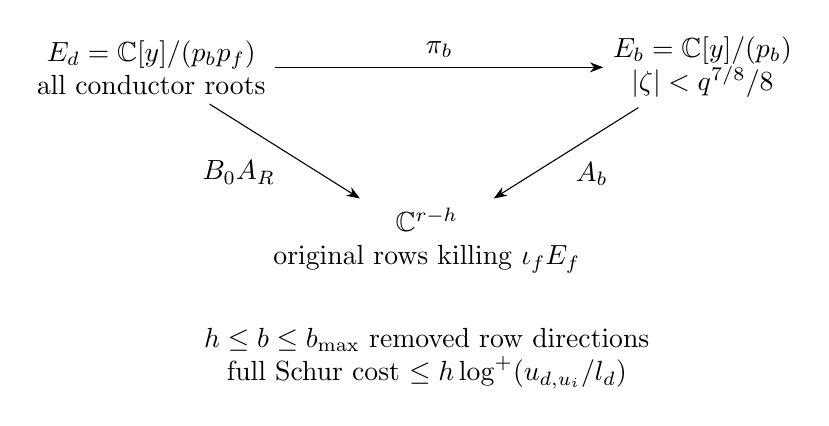
\begin{tikzpicture}[>=Stealth,every node/.style={align=center}]
\node (e) at (0,0) {$E_d=\C[y]/(p_bp_f)$\\all conductor roots};
\node (b) at (7,0) {$E_b=\C[y]/(p_b)$\\$|\zeta|<q^{7/8}/8$};
\node (o) at (3.5,-2.2) {$\C^{r-h}$\\original rows killing $\iota_fE_f$};
\draw[->] (e)--node[above] {$\pi_b$}(b);
\draw[->] (e)--node[below left] {$B_0A_R$}(o);
\draw[->] (b)--node[below right] {$A_b$}(o);
\node at (3.5,-3.7) {$h\le b\le b_{\max}$ removed row directions\\
full Schur cost $\le h\log^+(u_{d,u_i}/l_d)$};
\end{tikzpicture}
\caption{The exact factorization DCR5--8. The diagram uses the
original quotient and fixed observation. DCR10--19 evaluates the
retained return, and DCR20 pays for every complementary row.
The division circle defines primary factors with full multiplicity;
it is not a replacement of the physical root coordinates.
The complete final receiver is DCR22.}
\end{figure}

\begin{thebibliography}{9}
\bibitem{OOQ} Split-Zero research programme,
\emph{All directions of the original outer quotient at the leading scale},
OOQ1--40, with complete EIQ1--33 and OSP/OFV source proofs,
\href{https://github.com/KokunoYumeto/zeta-function-research-reader/blob/5992ad50c0f2a06921f1fcaded7b4e38097c0739/workbenches/splitzero-tandem/continuations/20260920-original-kernel-mixed-determinants/providers/09_INPUT_CUMULATIVE_PROOFS.tex#L23179}{pinned complete proof, OOQ section}.
The full OOQ section was read for this continuation; this does not
claim complete reading of the entire cumulative file.
\bibitem{OR} \emph{The roots of the complete conductor polynomial},
OR1--17,
\href{https://github.com/KokunoYumeto/zeta-function-research-reader/blob/0fd693c844aad9117e30ec447c59864a28af10f3/workbenches/splitzero-tandem/continuations/20260921-native-spectral-real-pair/003/COMPLETE_CONDUCTOR_ROOT_GEOMETRY.tex#L38}{pinned complete proof}.
\bibitem{CG} \emph{The complete conductor graph: a quantitative full-volume
comparison}, CG1--32, and \emph{The actual invariant kernel}, KF1--55,
\href{https://github.com/KokunoYumeto/zeta-function-research-reader/blob/0fd693c844aad9117e30ec447c59864a28af10f3/workbenches/splitzero-tandem/continuations/20260921-native-spectral-real-pair/003/COMPLETE_CONDUCTOR_GRAPH_METRIC.tex}{complete graph proof}.
\bibitem{CGR} \emph{The original invariant covariance and its conductor-pole
filtration}, CGR1--29, and \emph{The original strip has linear
elimination depth}, CGS1--22, 21 September 2026.
Complete proofs accompany this continuation; the publication must
include them before claiming a public proof-file link.
\bibitem{Human} J. L. W. V. Jensen,
\emph{Sur un nouvel et important th\'eor\`eme de la th\'eorie des fonctions},
Acta Mathematica 22 (1899), 359--364,
\href{https://doi.org/10.1007/BF02417878}{doi:10.1007/BF02417878}.
OR9 proves the needed zero-count formula completely.
The Gamma and orthogonal-polynomial identities used in the source
providers are due to the classical theory documented by R. A. Askey
and R. Roy, and by T. H. Koornwinder, R. Wong, R. Koekoek,
R. F. Swarttouw and W. P. Reinhardt in
\href{https://dlmf.nist.gov/5}{DLMF Chapter 5} and
\href{https://dlmf.nist.gov/18}{Chapter 18}.
No new external equilibrium theorem is imported here: the
equilibrium and polynomial estimates used are the full proved
programme sources linked above.
\end{thebibliography}

\end{document}
